%!TEX root = ../../paper.tex

% Ferdosi Set 2
\begin{subfigure}{0.23\textwidth}
	\centering
	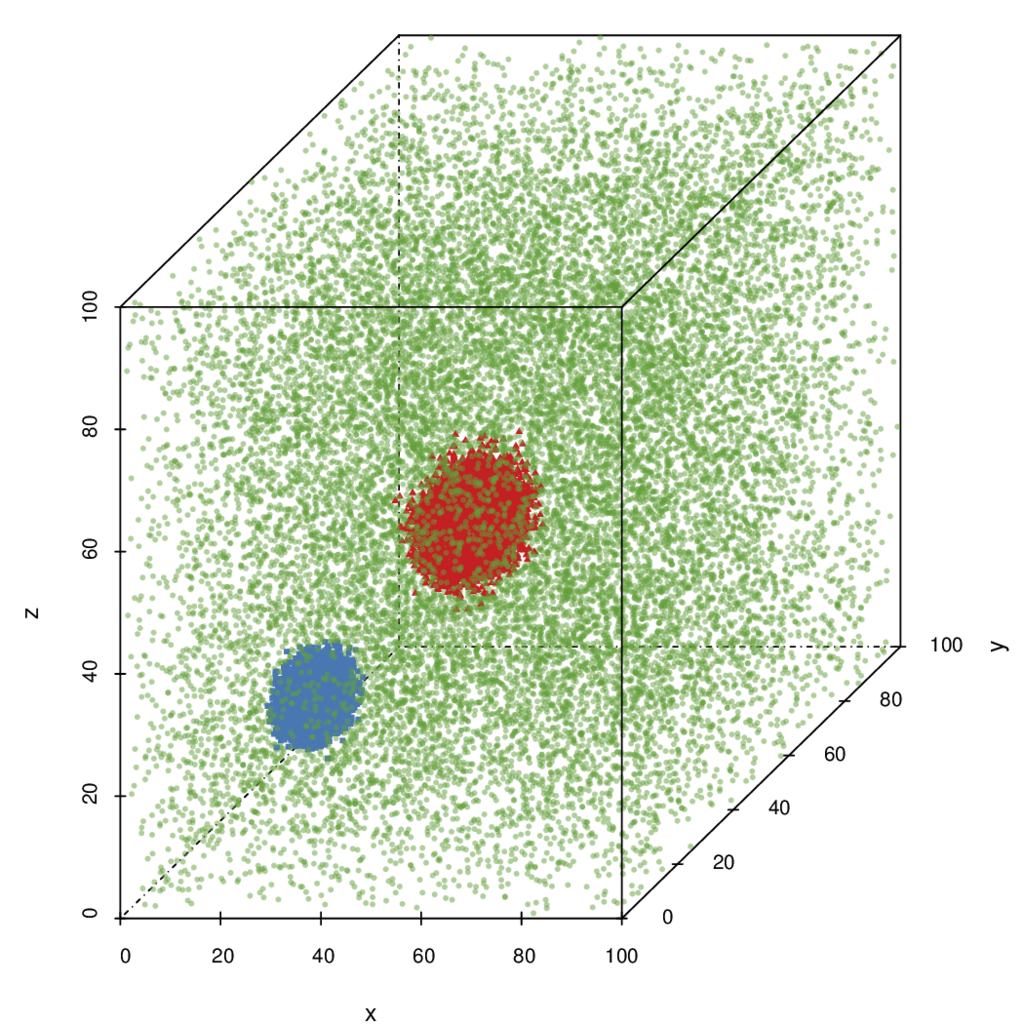
\includegraphics[width=\textwidth]{experiment/img/datasetplot_ferdosi_2_60000}
	\caption{Set \ferdosiTwo}
	\label{fig:experiment:multisphere:ferdosi2}
\end{subfigure}	
% Ferdosi Set 3
\begin{subfigure}{0.23\textwidth}
	\centering
	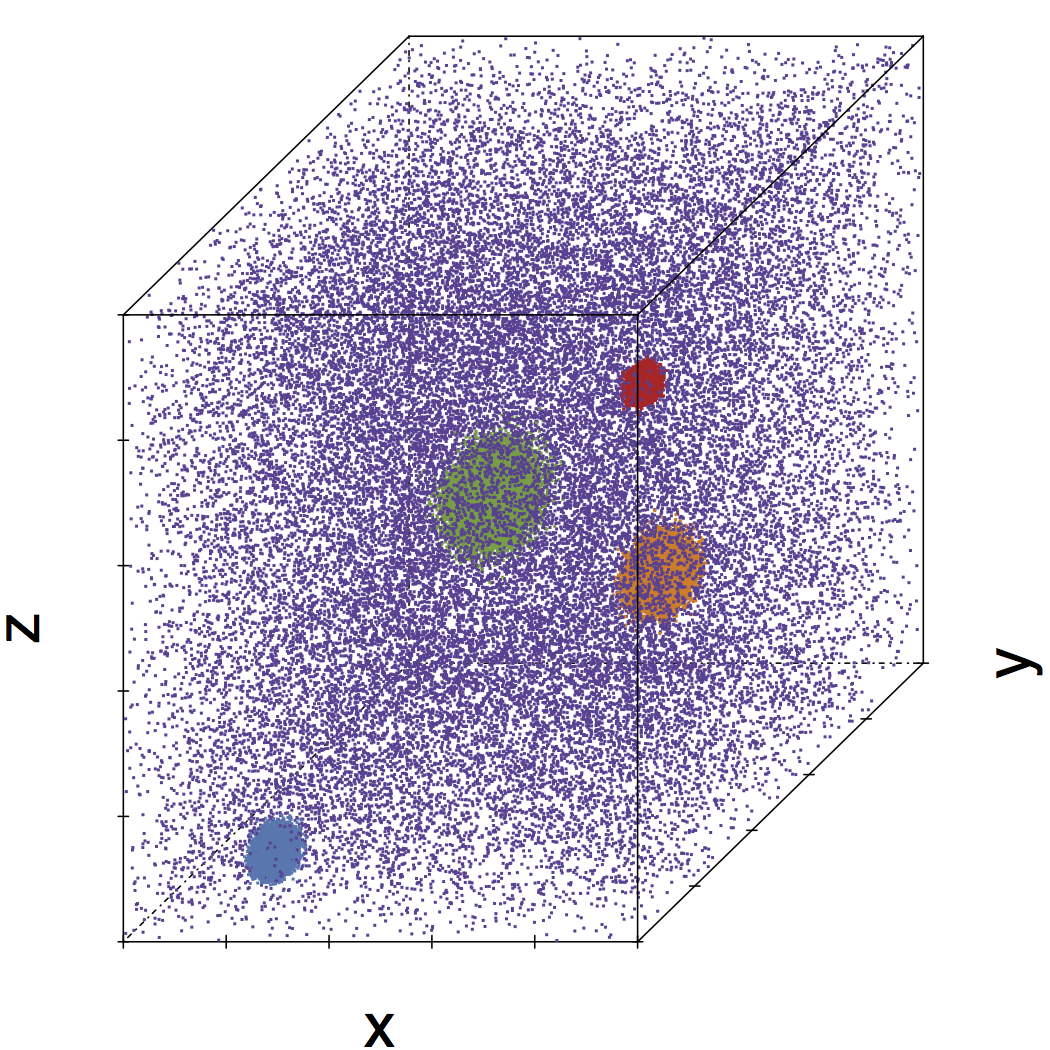
\includegraphics[width=\textwidth]{experiment/img/datasetplot_ferdosi_3_120000}
	\caption{Set \ferdosiThree}
	\label{fig:experiment:multisphere:ferdosi3}
\end{subfigure}	
\subfigvspace
% Baakman 2
\begin{subfigure}{0.23\textwidth}
	\centering
	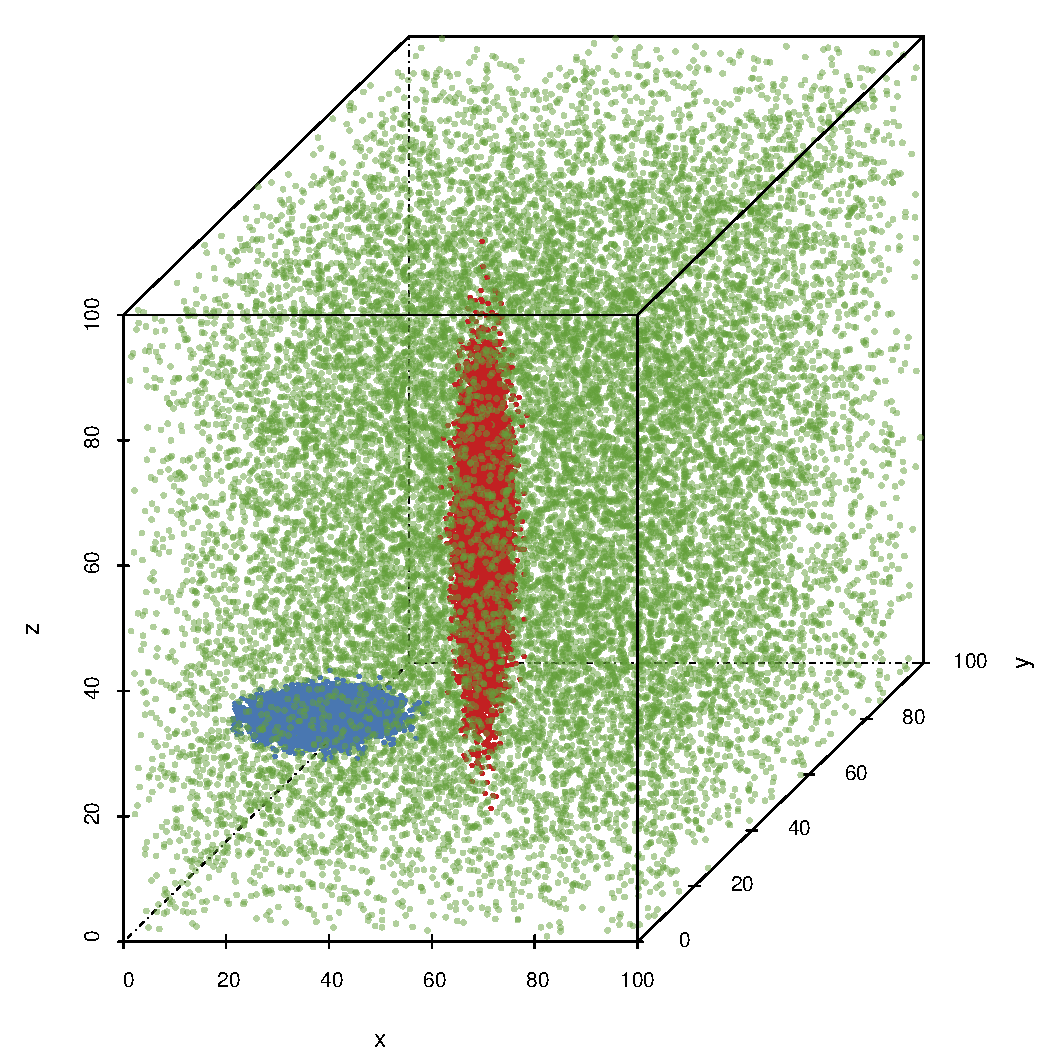
\includegraphics[width=\textwidth]{experiment/img/datasetplot_baakman_2_60000}
	\caption{Set \baakmanTwo}
	\label{fig:experiment:multisphere:baakman2}
\end{subfigure}			
% Baakman 3
\begin{subfigure}{0.23\textwidth}
	\centering
	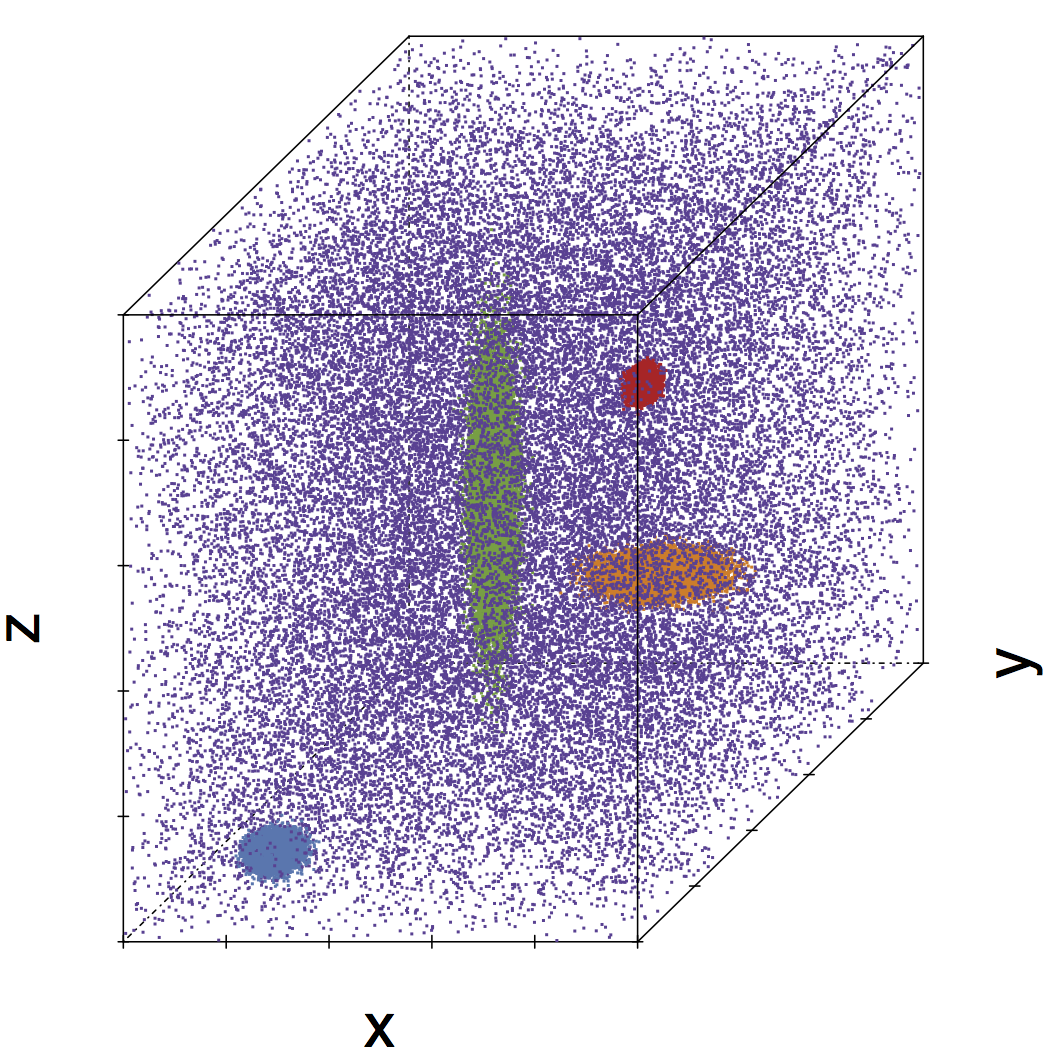
\includegraphics[width=\textwidth]{experiment/img/datasetplot_baakman_3_120000}
	\caption{Set \baakmanThree}
	\label{fig:experiment:multisphere:baakman3}
\end{subfigure}